\chapter{Testing and Results}
Much of this project revolved around testing of the capability of Bluetooth Low Energy, iBeacon, iPhone and the feasibility of using these technologies in tandem to crate a positioning system that could perform with useful accuracy.  As mentioned in 4.4.1, most of the testing and calibration was done in two dimensions.  This was accomplished by using a large printed grid for testing in a smaller area, and measured distances in a large room for testing on a larger scale.  In order to determine the feasibility of the iBeacons for location tracking, it was important to determine the accuracy with which the distance between the iOS device and the iBeacon could be determined.  This distance is derived from the Received Signal Strength Indicator (RSSI) value which is measured in decibels.  In order to understand how effectively the RSSI can be translated into a measure of distance, we build a testing App that could record a variety of data about different RSSI values, and export them for further analysis.  A screenshot of this testing App can be seen in Appendix C.

One of the questions that needed answering for this project was which type of iBeacons would be sufficient for the system.  The main factor to consider is the broadcast power of the iBeacon.  In order to see what effect power had on the relationship between RSSI and distance from the beacon, we placed a series of beacons at known locations.  We then recorded the relationship between RSSI and distance at a variety of locations for a set of low powered beacons and then again with higher powered ones.  These relationships are visually displayed in the figures below.

\begin{figure}[h]
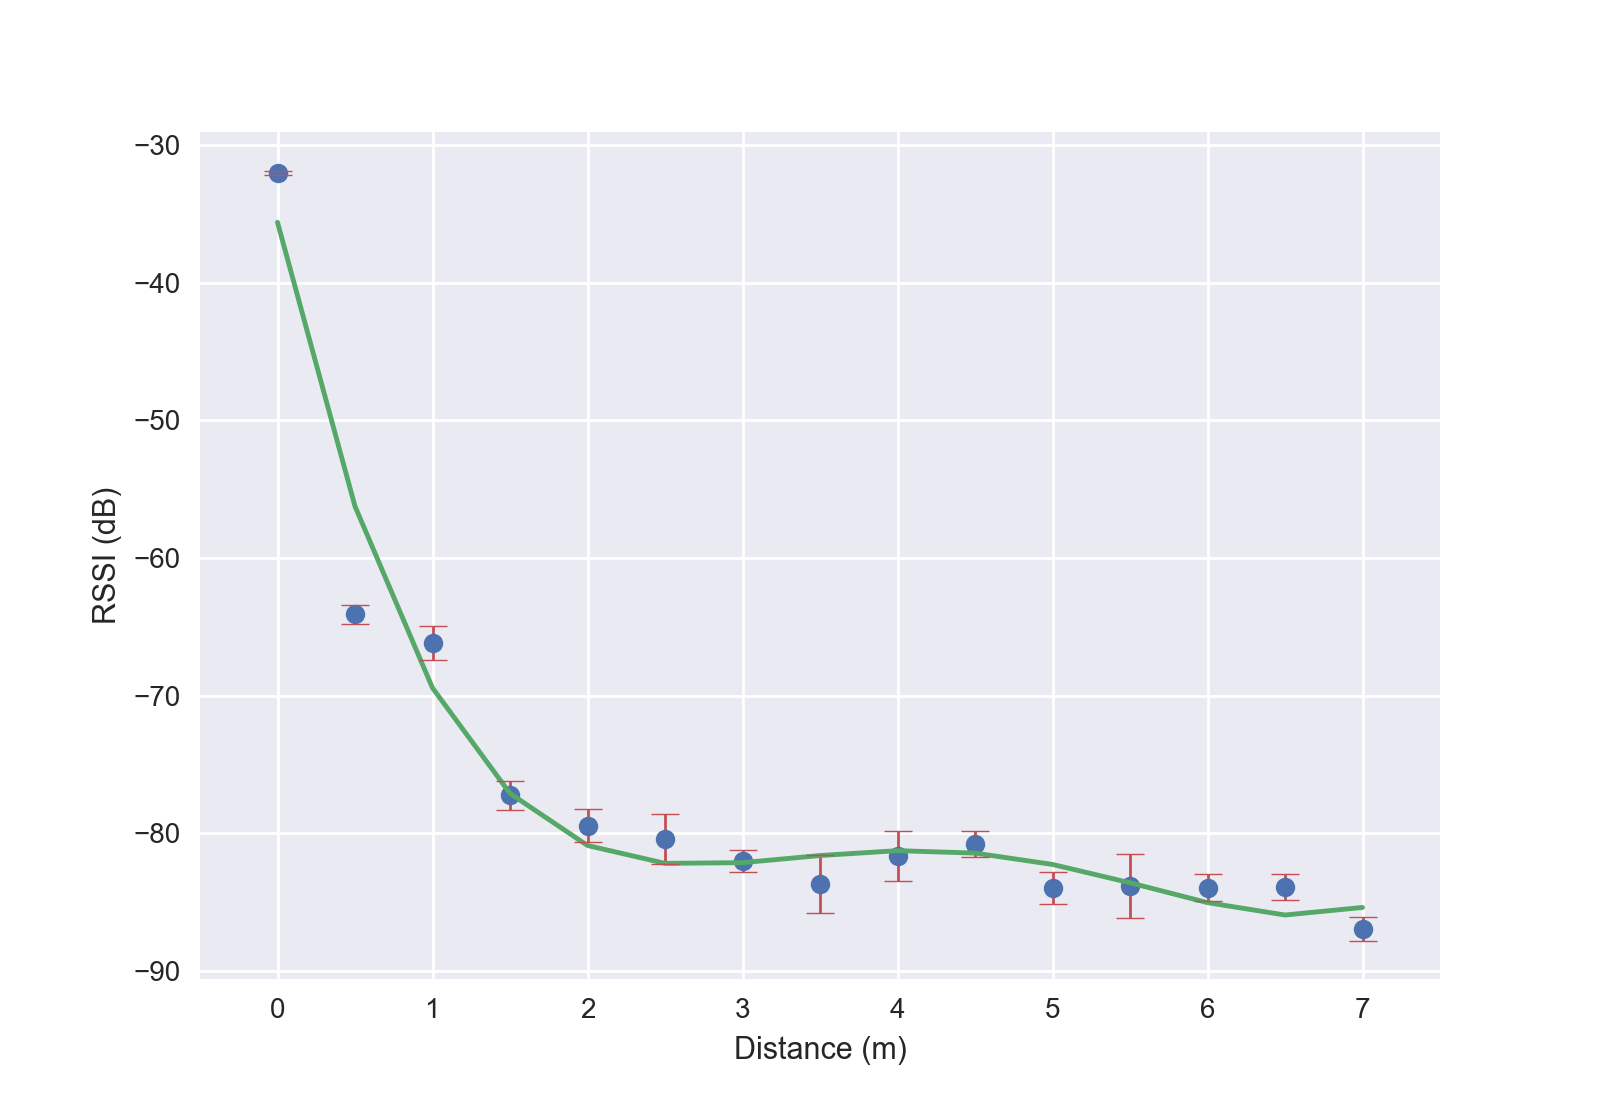
\includegraphics[width=.85\textwidth]{images/Oltica.png}
\caption{RSSI v. distance - low powered beacon}
\vspace{1em}
Figure 5.1 shows that the relationship between RSSI and distance is meaningful up to about two meters away from the low powered beacon.
\end{figure}

\begin{figure}[h]
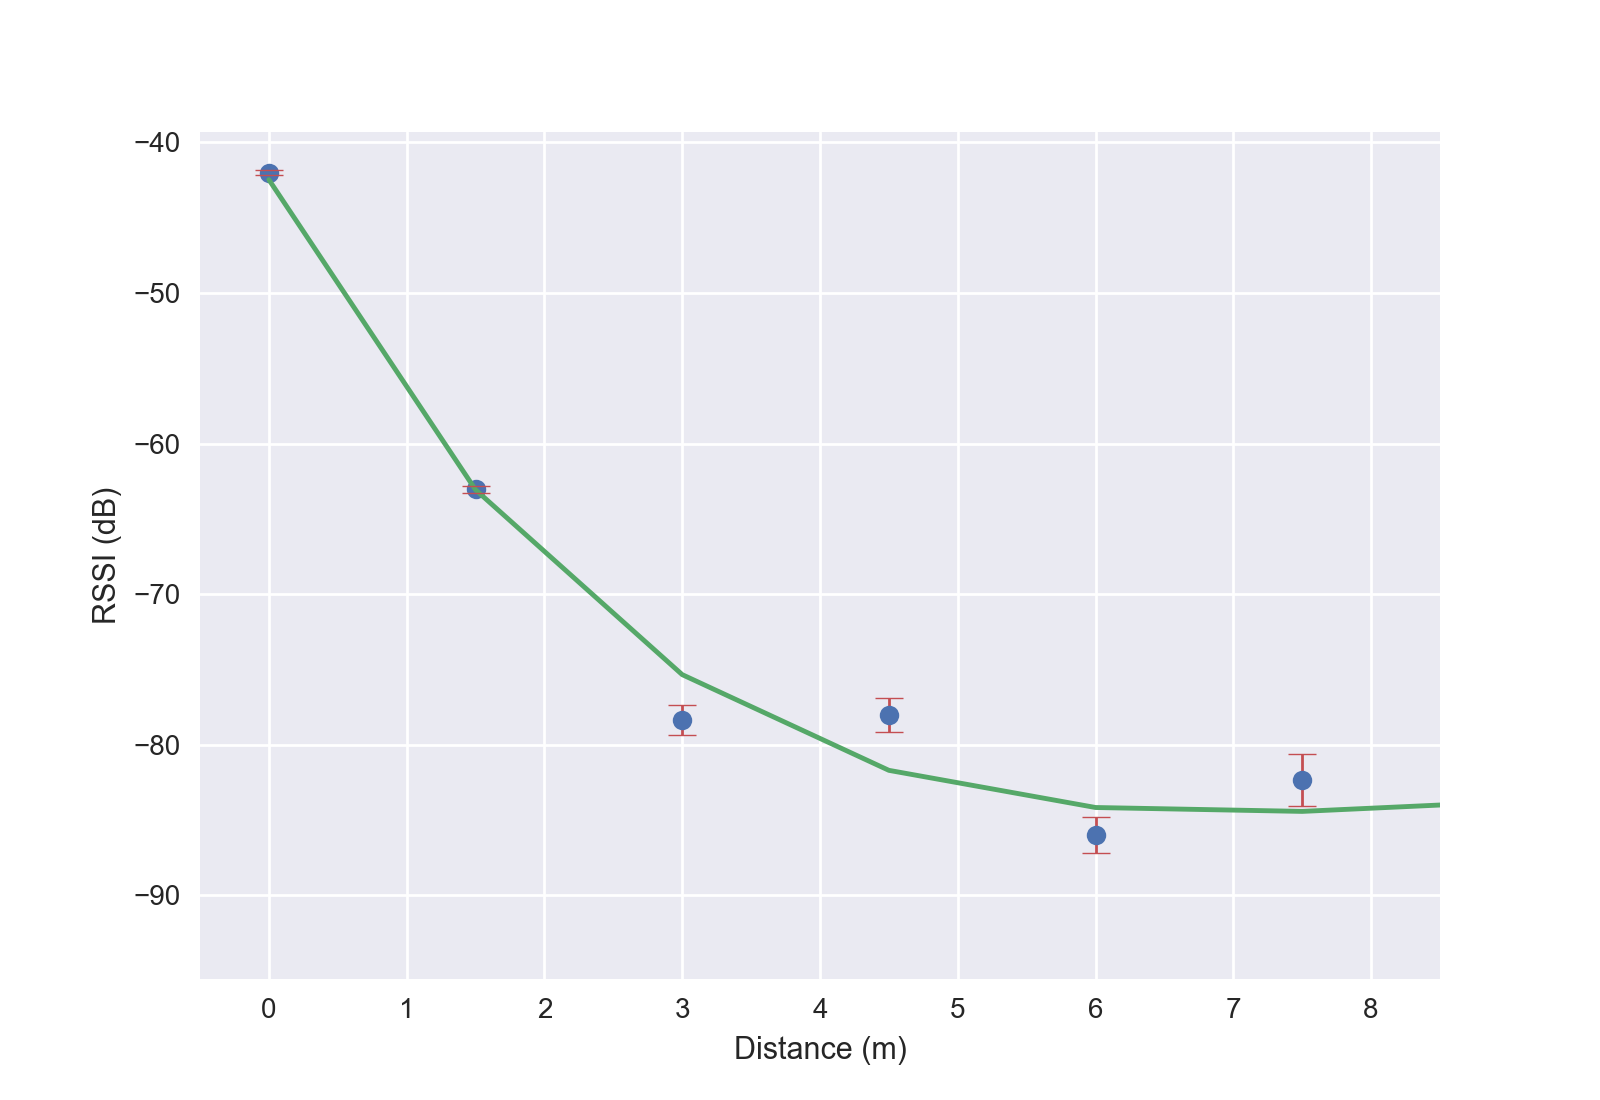
\includegraphics[width=.85\textwidth]{images/Estimote.png}
\caption{RSSI v. distance - high powered beacon}
\vspace{1em}
Figure 5.2 shows that the relationship between RSSI and distance is meaningful up to about four meters away from the higher powered beacon.
\end{figure}

These tests of the RSSI values revealed that a set of higher powered beacon would be necessary to cover any significantly large area.  However, it should be noted that while these measurements of distance represent the r values used in the trilateration algorithm described in 4.4.1, when considering usable coverage of the beacon in the system, that value should be doubled.  This is because the area of coverage is represented by the diameter of the usable broadcast circle.  This is due to the omnidirectional nature of the BLE antenna on most iBeacon broadcast devices.

The iBeacon broadcast packet contains not only the RSSI value but also unique identifiers that allows the BLE Location framework to associate each signal with a known beacon location.  Assuming a device is within the meaningful broadcast range of three or more beacons, this associated set of locations, combined with the translated RSSI values, provides enough information to the framework for it to make an estimation of location.  This location is relative to the coordinate plane defined during the configuration stage, but can be translated back into latitude and longitude using conversion factors provided by the framework API.  By placing beacons at known locations, and moving iOS devices running the test application we were able to get a feel for the general accuracy of the system when using low powered beacons, or higher powered ones.
